\documentclass[11pt]{article}

\usepackage[margin=1in]{geometry}
\usepackage{amsmath,amssymb,amsthm}
\usepackage{mathtools}
\usepackage{enumitem}
\usepackage{tikz}
\usetikzlibrary{calc,positioning}
\usepackage[colorlinks=true,linkcolor=blue!50!black,citecolor=blue!50!black,urlcolor=blue!50!black]{hyperref}

\newtheorem{theorem}{Theorem}[section]
\newtheorem{proposition}[theorem]{Proposition}
\newtheorem{lemma}[theorem]{Lemma}
\newtheorem{corollary}[theorem]{Corollary}
\newtheorem{conjecture}[theorem]{Conjecture}
\theoremstyle{definition}
\newtheorem{definition}[theorem]{Definition}
\newtheorem{example}[theorem]{Example}
\newtheorem{remark}[theorem]{Remark}

\newcommand{\X}{\mathbf{X}}
\newcommand{\St}{\mathbf{S}}
\newcommand{\K}{\mathbf{K}}
\newcommand{\PP}{\mathbb{P}}
\newcommand{\NN}{\mathbb{N}}
\newcommand{\ZZ}{\mathbb{Z}}
\newcommand{\type}{\operatorname{type}}
\newcommand{\diam}{\operatorname{diam}}
\newcommand{\deglow}{\operatorname{deg}}

\title{On Distinguishing Trees by Their Chromatic Symmetric Functions: \\
       \large A Report on Martin--Morin--Wagner}
\author{Math 725 Independent Project}
\date{}

\begin{document}
\maketitle

\begin{abstract}
This report is an exposition of, and a small extension to, the paper
\emph{On Distinguishing Trees by Their Chromatic Symmetric Functions}
by J.~L.~Martin, M.~Morin, and J.~D.~Wagner~\cite{MMW}.  The central
question, raised by Stanley~\cite{Stanley}, is whether the chromatic
symmetric function $\X_T$ is a complete isomorphism invariant on the
class of trees.  After developing the necessary background, we present
a complete proof, in our own words, of the paper's caterpillar
reconstruction theorem (Theorem~\ref{thm:cat}), which shows that
caterpillars with strictly positive and pairwise distinct leaf numbers
are determined up to isomorphism by their chromatic symmetric functions.
We then work out two examples in detail and propose a strengthening of
the paper's main open question, supported by computational evidence and
a partial result.
\end{abstract}

\section{Introduction}\label{sec:intro}

A central theme in algebraic graph theory is the search for combinatorial
invariants that distinguish graphs up to isomorphism.  The
\emph{chromatic polynomial} $\chi_G(k)$, which counts proper colorings of
$G$ with at most $k$ colors, is well known but extremely weak on trees:
every tree on $n$ vertices satisfies $\chi_T(k)=k(k-1)^{n-1}$, so the
chromatic polynomial cannot distinguish two non-isomorphic trees.
In~1995, Stanley~\cite{Stanley} introduced a much finer invariant.

\begin{definition}\label{def:csf}
Let $G=(V,E)$ be a finite simple graph.  The
\emph{chromatic symmetric function} of $G$ is
\[
   \X_G(x_1,x_2,\ldots) \;=\; \sum_{\kappa}\;\prod_{v\in V} x_{\kappa(v)},
\]
where the sum runs over all proper colorings $\kappa\colon V\to \PP$ of $G$
by positive integers.  Permuting the variables permutes the colorings,
so $\X_G$ is a symmetric function, homogeneous of degree $|V|$.
\end{definition}

The chromatic polynomial is recovered from $\X_G$ by setting
$x_1=\cdots=x_k=1$ and $x_i=0$ for $i>k$.  Thus $\X_G$ refines the
chromatic polynomial.  Stanley showed that $\X_G$ is \emph{not} a
complete isomorphism invariant on graphs in general, exhibiting two
non-isomorphic five-vertex graphs with the same chromatic symmetric
function~\cite{Stanley}.  Whether $\X_T$ is a complete invariant on the
restricted class of \emph{trees} remains open and is one of the most
prominent unsolved problems in algebraic combinatorics.  The source
paper cites Tan's computational verification through $23$ vertices;
later work of Heil and Ji extends this verification through $29$
vertices~\cite{Tan,HeilJi}.

The paper of Martin, Morin, and Wagner~\cite{MMW} attacks this question
from two complementary angles.  First, they show that $\X_T$ is at least
as strong an invariant as the \emph{subtree polynomial} $\St_T(q,r)$,
which is the bivariate generating function counting subtrees of $T$ by
their numbers of edges and leaves.  In particular, the path and degree
sequences of $T$ can be extracted from $\X_T$.  Second, they prove that
$\X_T$ \emph{does} reconstruct $T$ when $T$ is restricted to certain
natural sub-classes, including all spiders, several families of
caterpillars, and (in the unicyclic setting) all squids.
The paper's main theorem, which recovers the subtree and connector
polynomials from $\X_T$, is the main engine behind these results: it
shows that $\X_T$ remembers many ordinary structural statistics of a
tree.  The caterpillar theorem proved below is a more refined application
of the same coefficient data, using the special way edge subsets sit
inside a caterpillar.

The remainder of this report is organized as follows.
Section~\ref{sec:prelim} fixes notation and reviews symmetric-function
preliminaries.  Section~\ref{sec:expansion} states Stanley's power-sum
expansion of $\X_G$ and explains why it is especially well-behaved on
trees.  Section~\ref{sec:invariants} catalogs the basic graph invariants
recoverable from $\X_T$.  Section~\ref{sec:thm} contains the main
theorem of this report---a caterpillar reconstruction theorem due to
Martin--Morin--Wagner---together with a complete, self-contained proof
in our own words.  Section~\ref{sec:examples} works out two original
examples.  Section~\ref{sec:conjecture} states a conjecture, supported
by partial results, and Section~\ref{sec:code} briefly comments on
computational verification.

\section{Preliminaries on symmetric functions and trees}\label{sec:prelim}

We follow~\cite{Macdonald,StanleyEC2} for symmetric functions
and~\cite{Bollobas} for graphs.

\paragraph{Partitions.}
A \emph{partition} of $n$ is a weakly decreasing sequence
$\lambda = (\lambda_1\geq\lambda_2\geq\cdots\geq\lambda_\ell)$ of
positive integers summing to $n$.  We write $\lambda\vdash n$.  The
number $\ell=\ell(\lambda)$ is the \emph{length} of $\lambda$.  We say
$\lambda$ is \emph{singleton-free} if every part is $\geq 2$.

\paragraph{Power-sum symmetric functions.}
For each $k\in\PP$ define $p_k = \sum_{i\geq 1} x_i^k$, and for a
partition $\lambda$ set $p_\lambda = \prod_{j=1}^{\ell(\lambda)}
p_{\lambda_j}$.  The set $\{p_\lambda : \lambda\vdash n\}$ is a
$\mathbb{Q}$-vector-space basis for the space $\Lambda^n$ of
homogeneous symmetric functions of degree~$n$.

\paragraph{Trees.}
A \emph{tree} $T=(V,E)$ is a connected graph with $|E|=|V|-1$; equivalently,
a connected acyclic graph.  A \emph{leaf} is a vertex of degree~$1$, and
the unique edge incident to a leaf is a \emph{leaf edge}.  We write
$\delta_j(T)$ for the number of degree-$j$ vertices of $T$, and
$\pi_i(T)$ for the number of paths in $T$ with exactly $i$ edges.

\paragraph{Caterpillars.}
A \emph{caterpillar} is a tree whose non-leaf vertices induce a
nontrivial path, called the \emph{spine}.  We label the spine as
$v_0,v_1,\ldots,v_s$ (so it has $s+1$ vertices and $s$ edges), and
denote by $f_i$ the number of leaves attached to $v_i$, called the
\emph{$i$-th leaf number} of $T$.  Note that $f_0,f_s\geq 1$ (otherwise
$v_0$ or $v_s$ would itself be a leaf and not lie on the spine), but
$f_i$ for $0<i<s$ may be zero.

\section{Stanley's expansion and tree-specific structure}\label{sec:expansion}

The starting point of~\cite{MMW} is the following expansion of $\X_G$
due to Stanley~\cite[Thm.~2.5]{Stanley}.

\begin{theorem}[Stanley's expansion]\label{thm:stanley}
For any finite graph $G=(V,E)$,
\begin{equation}\label{eq:expansion}
   \X_G \;=\; \sum_{A\subseteq E} (-1)^{|A|}\,p_{\type(A)},
\end{equation}
where $\type(A)$ is the partition whose parts are the orders of the
connected components of the spanning subgraph $(V,A)$.
\end{theorem}

We write $c_\lambda(G)$ for the coefficient of $p_\lambda$ in the
power-sum expansion of $\X_G$, so that
$\X_G = \sum_{\lambda\vdash n} c_\lambda(G)\,p_\lambda$.

When $G=T$ is a tree, every $A\subseteq E(T)$ is acyclic, so the
spanning subgraph $(V,A)$ has exactly $n-|A|$ components, and hence
$\ell(\type(A)) = n-|A|$.  In particular all edge subsets of a fixed
type contribute the same sign $(-1)^{|A|}$, and we obtain the clean
formula
\begin{equation}\label{eq:tree-cl}
   c_\lambda(T)
   \;=\;(-1)^{n-\ell(\lambda)}
        \cdot \bigl|\{A\subseteq E(T) : \type(A)=\lambda\}\bigr|.
\end{equation}
Equation~\eqref{eq:tree-cl} is the combinatorial linchpin of the entire
paper, and we shall use it repeatedly.

\section{Recovering classical invariants}\label{sec:invariants}

We summarize the basic invariants of a graph (or tree) that are
captured by $\X_G$, following~\cite[Prop.~2 \& Cor.~5]{MMW}.

\begin{proposition}\label{prop:invariants}
For any graph $G=(V,E)$, the chromatic symmetric function $\X_G$
determines:
\begin{enumerate}[label=\textup{(\roman*)}]
   \item the number of vertices, $n=|V|$;
   \item the number of edges, $|E| = -c_{(2,1,1,\ldots,1)}(G)$;
   \item the number of connected components,
         $\min\{\ell(\lambda) : c_\lambda(G)\neq 0\}$.
\end{enumerate}
If $T$ is a tree, then $\X_T$ also determines:
\begin{enumerate}[label=\textup{(\roman*)},resume]
   \item the number of $j$-vertex subtrees, namely
         $\bigl|c_{(j,1,\ldots,1)}(T)\bigr|$ for each $j\geq 2$;
   \item the number of leaves of $T$, namely
         $|c_{(n-1,1)}(T)|$;
   \item the path sequence $(\pi_i(T))_{i\geq 1}$ and the degree
         sequence $(\delta_j(T))_{j\geq 1}$.
\end{enumerate}
\end{proposition}

The recovery of the path and degree sequences is in fact a corollary of
the much stronger result of Martin--Morin--Wagner that the
\emph{subtree polynomial}
\(
   \St_T(q,r) = \sum_S q^{|E(S)|}\,r^{|L(S)|},
\)
where the sum is over edge-nonempty subtrees $S$ of $T$ and $L(S)$
denotes the leaf edges of $S$, can be extracted from $\X_T$ by an
explicit linear formula~\cite[Thm.~1]{MMW}.  The path sequence appears
as the coefficients of $q^i r^2$ in $\St_T$, and the star sequence
(equivalent to the degree sequence) as the coefficients of $q^k r^k$.

\section{The main theorem: caterpillars with distinct leaf numbers}\label{sec:thm}

The principal result we shall prove is the caterpillar reconstruction
theorem of~\cite[Thm.~11]{MMW}.  It illustrates beautifully how the
combinatorial interpretation~\eqref{eq:tree-cl} of $c_\lambda(T)$ on
trees converts a structural question---``which tree is $T$?''---into
the combinatorial problem of identifying which edge-subsets realize
which types.

\begin{theorem}[Martin--Morin--Wagner]\label{thm:cat}
Let $T$ be a caterpillar with spine $v_0,v_1,\ldots,v_s$ and leaf
numbers $f_0,f_1,\ldots,f_s$.  Suppose every $f_i$ is strictly positive
and that the $f_i$ are pairwise distinct.  Then $T$ is determined up to
isomorphism by its chromatic symmetric function $\X_T$.
\end{theorem}

\begin{proof}
Fix the caterpillar $T$ as in the statement, and set
$n = |V(T)| = (s+1) + \sum_{i=0}^{s} f_i$ and
$L \subseteq E(T)$ the set of leaf edges of $T$.  Write
$E_{\mathrm{spine}} = \{e_1,\ldots,e_s\}$ for the spine edges, where
$e_i = v_{i-1}v_i$.  Throughout, partitions are equated with their
multisets of parts.

We will show that the data
\[
  \mathcal{D}(T) \;:=\; \bigl\{c_\lambda(T) : \lambda\vdash n\bigr\}
\]
suffices to recover $(f_0,f_1,\ldots,f_s)$ up to reversal.  The
isomorphism type of $T$ depends only on this sequence up to reversal
(reflecting the spine end-to-end produces an isomorphic caterpillar),
so this is enough.

\medskip\noindent
\textbf{Step 1: Edge subsets with singleton-free type are exactly
the supersets of $L$.}
Suppose $A\subseteq E(T)$ has $\type(A)$ singleton-free, i.e.\ every
component of the spanning subgraph $(V,A)$ has order $\geq 2$.  In
particular, every leaf $w$ of $T$ lies in a component of size $\geq 2$,
which forces $A$ to contain the unique edge incident to $w$.  Hence
$L\subseteq A$.

Conversely, if $A\supseteq L$, then for every spine vertex $v_i$ the
component of $(V,A)$ containing $v_i$ contains at least the $f_i\geq 1$
leaves attached to $v_i$ together with $v_i$ itself, so it has order
$\geq f_i+1\geq 2$.  Every leaf is also in such a component (the same
one as its spine neighbor), so every component has order $\geq 2$ and
$\type(A)$ is singleton-free.

Consequently, edge sets $A$ contributing to a singleton-free
$c_\lambda(T)$ are precisely those of the form $A = L\cup B$ with
$B\subseteq E_{\mathrm{spine}}$.

\medskip\noindent
\textbf{Step 2: Identifying $\lambda := \type(L)$.}
Starting from the spanning subgraph $(V,L)$, the $s+1$ nontrivial
components have vertex sets $\{v_i\}$ together with the leaves attached
to $v_i$.  Adding the $|B|$ spine edges in $B$ merges exactly $|B|$
adjacent pairs of these components, since the spine is a path and hence
$B$ is acyclic.  Therefore
$\ell(\type(L\cup B)) = (s+1)-|B|$, and the maximum length is achieved
exactly when $B=\emptyset$.

Set $\lambda := \type(L)$.  Then $\lambda$ has parts $f_0+1, f_1+1,
\ldots, f_s+1$ (one for each spine vertex).  Step~1 and the preceding
paragraph show:
\[
   \lambda \text{ is the \emph{unique} singleton-free partition of $n$
   of length $s+1$ with } c_\lambda(T)\neq 0,
\]
and indeed $c_\lambda(T) = (-1)^{n-(s+1)}$ since exactly one edge set
($A=L$ itself) has type $\lambda$.  We can read off $s+1$ as the
maximum length of a singleton-free partition appearing in
$\X_T$ with nonzero coefficient, and then $\lambda$ as the unique such
partition of that length.  In particular, the multiset
$\{f_0+1,f_1+1,\ldots,f_s+1\}$, hence the multiset
$\{f_0,f_1,\ldots,f_s\}$, is determined by $\X_T$.

Note that since the $f_i$ are pairwise distinct, all parts of $\lambda$
are pairwise distinct.

\medskip\noindent
\textbf{Step 3: Identifying the partitions $\mu_i := \type(L\cup\{e_i\})$.}
Now consider $|B|=1$, say $B = \{e_i\}$.  The edge $e_i = v_{i-1}v_i$
merges precisely the two components of $(V,L)$ containing $v_{i-1}$ and
$v_i$, of sizes $f_{i-1}+1$ and $f_i+1$, into a single component of
size $f_{i-1}+f_i+2$; the other $s-1$ components are unaffected.  Hence
\[
   \mu_i \;:=\; \type(L\cup\{e_i\})
   \;=\; \bigl(\,\lambda \setminus \{f_{i-1}+1,\;f_i+1\}\,\bigr)
         \,\cup\, \{f_{i-1}+f_i+2\},
\]
where we manipulate $\lambda$ as a multiset of parts.

By Step~1 and the length count from Step~2, the edge subsets with
$\type$ singleton-free of length exactly $s$ are precisely
$L\cup\{e_1\},\ldots,L\cup\{e_s\}$.  Thus the relevant partitions are
exactly $\mu_1,\ldots,\mu_s$, counted with multiplicity.  We next explain
why, under the distinctness hypothesis, each $\mu_i$ identifies the
corresponding unordered adjacent pair of leaf numbers.

Since the parts of $\lambda$ are pairwise distinct, the multiset
difference between $\lambda$ and the largest common submultiset of
$\lambda$ and $\mu_i$ consists of exactly the two deleted parts
$f_{i-1}+1$ and $f_i+1$.  This remains true even if the new part
$f_{i-1}+f_i+2$ happens to equal another part of $\lambda$, because we
compare multisets with multiplicity.  Therefore $\mu_i$ determines the
unordered pair
\[
   \{f_{i-1}+1,\,f_i+1\},
\]
and hence determines the unordered pair $\{f_{i-1},f_i\}$.

If two different spine edges produced the same partition $\mu$, the
preceding paragraph would give the same unordered pair of leaf numbers
for both edges.  Since the $f_k$ are pairwise distinct, that unordered
pair occurs for only one edge of the path.  Hence the partitions
$\mu_1,\ldots,\mu_s$ are pairwise distinct, and the set
$\{\mu_1,\ldots,\mu_s\}$ is determined by $\X_T$ as the set of
singleton-free partitions $\mu$ of $n$ with $\ell(\mu)=s$ and
$c_\mu(T)\neq 0$.

\medskip\noindent
\textbf{Step 4: Reconstructing the leaf-number sequence.}
From each partition $\mu_i$, compare it with $\lambda$ as a multiset and
record the two parts of $\lambda$ that are deleted.  Subtracting $1$
from those two parts gives exactly the unordered adjacent pair
$\{f_{i-1},f_i\}$.

Form an auxiliary graph $H$ on the vertex set
$V(H) = \{f_0,f_1,\ldots,f_s\}$ (a set of $s+1$ \emph{distinct}
non-negative integers, by hypothesis) with edges
$E(H) = \{\{f_{i-1},f_i\} : 1\leq i\leq s\}$.  Steps~2 and~3 show that
$V(H)$ and $E(H)$ are determined by $\X_T$.  But $H$ is the path
$f_0$--$f_1$--$\cdots$--$f_s$ on $s+1$ vertices, and a path on labeled
vertices is determined up to reversal by its edge set.  Hence the
sequence $(f_0,\ldots,f_s)$ is determined by $\X_T$ up to reversal,
which (as noted above) determines the caterpillar $T$ up to isomorphism.
\end{proof}

\begin{remark}\label{rem:relax}
The hypothesis that the $f_i$ are pairwise distinct can be weakened.
The argument in Step~3 only used distinctness to ensure that whenever
$\mu_i = \mu_j$ one has $\{f_{i-1},f_i\} = \{f_{j-1},f_j\}$.  If we
instead assume that for each value $k$, the set
$\{i : f_i = k\}$ forms a contiguous subpath of indices, then the
argument still allows us to identify which adjacencies $\{f_{i-1},f_i\}$
appear as multisets, and hence to reconstruct~$T$.  This relaxation is
mentioned in passing in~\cite[\S 4]{MMW}.
\end{remark}

\section{Worked examples}\label{sec:examples}

We work two examples that do not appear in~\cite{MMW}.  The first
explicitly computes the chromatic symmetric function of a small tree
and verifies the identities of Proposition~\ref{prop:invariants}.  The
second illustrates Theorem~\ref{thm:cat} on a caterpillar with three
spine vertices.

\subsection{Example: full power-sum expansion of a five-vertex tree}\label{ex:1}

Let $T$ be the tree on $n=5$ vertices with vertex set
$\{v_0,v_1,\ell_0,\ell_1,\ell_1'\}$ and edge set
$E(T) = \{e_1,e_2,e_3,e_4\}$, where
\[
   e_1 = v_0v_1,\quad
   e_2 = v_0\ell_0,\quad
   e_3 = v_1\ell_1,\quad
   e_4 = v_1\ell_1'.
\]
Equivalently, $T$ is the caterpillar with spine $v_0,v_1$ and leaf
numbers $f_0=1$, $f_1=2$, or equivalently the spider $T_{(2,1,1)}$.
A picture is shown below.

\begin{center}
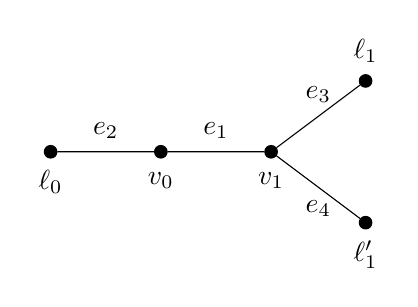
\begin{tikzpicture}[every node/.style={circle,draw,inner sep=1.6pt,fill=black}]
   \node[label=below:{$\ell_0$}] (l0) at (0,0) {};
   \node[label=below:{$v_0$}]    (v0) at (1.4,0) {};
   \node[label=below:{$v_1$}]    (v1) at (2.8,0) {};
   \node[label=above:{$\ell_1$}] (l1) at (4.0,0.9) {};
   \node[label=below:{$\ell_1'$}](l1p) at (4.0,-0.9) {};
   \draw (l0) -- node[draw=none,fill=none,above]{$e_2$} (v0)
              -- node[draw=none,fill=none,above]{$e_1$} (v1)
              -- node[draw=none,fill=none,above]{$e_3$} (l1);
   \draw (v1) -- node[draw=none,fill=none,below]{$e_4$} (l1p);
\end{tikzpicture}
\end{center}

We compute $\X_T = \sum_{A\subseteq E(T)} (-1)^{|A|}\,p_{\type(A)}$ by
enumerating all $2^4=16$ edge subsets $A\subseteq E(T)$ and tabulating
their types.

\begin{center}
\begin{tabular}{c|c|c|c}
$|A|$ & subsets & component sizes & type \\\hline
$0$  & $\varnothing$
     & five singletons          & $(1^5)$ \\
$1$  & each of $\{e_1\},\{e_2\},\{e_3\},\{e_4\}$
     & one edge plus 3 isolated   & $(2,1,1,1)$ \\
$2$  & $\{e_1,e_2\},\{e_1,e_3\},\{e_1,e_4\},\{e_3,e_4\}$
     & one $P_3$ plus 2 isolated  & $(3,1,1)$ \\
$2$  & $\{e_2,e_3\},\{e_2,e_4\}$
     & two edges plus 1 isolated  & $(2,2,1)$ \\
$3$  & $\{e_1,e_2,e_3\},\{e_1,e_2,e_4\},\{e_1,e_3,e_4\}$
     & one $P_4$/star plus 1      & $(4,1)$ \\
$3$  & $\{e_2,e_3,e_4\}$
     & disjoint $P_2$ and $P_3$   & $(3,2)$ \\
$4$  & $E(T)$
     & all of $T$                 & $(5)$ \\
\end{tabular}
\end{center}

Tallying the signed contributions to each $c_\lambda(T)$ gives
\begin{align}
   \X_T \;=\;\;& p_{(1,1,1,1,1)} \;-\; 4\,p_{(2,1,1,1)} \;+\; 4\,p_{(3,1,1)}
              \;+\; 2\,p_{(2,2,1)} \nonumber\\
              & \;-\; 3\,p_{(4,1)} \;-\; p_{(3,2)} \;+\; p_{(5)}.
   \label{eq:XT5}
\end{align}

We now verify each part of Proposition~\ref{prop:invariants}:
\begin{enumerate}[label=\textup{(\roman*)}]
   \item Every monomial of every $p_\lambda$ in~\eqref{eq:XT5} has
         total degree $5 = |V(T)|$.
   \item $-c_{(2,1,1,1)}(T) = -(-4) = 4 = |E(T)|$.
   \item The minimum length of a partition with non-zero coefficient
         is $\ell((5)) = 1$, matching the $1$ component of $T$.
   \item For $j=3$ we have $|c_{(3,1,1)}(T)| = 4$, and indeed $T$ has
         $4$ subtrees on $3$ vertices: the three paths
         $\ell_0v_0v_1$, $v_0v_1\ell_1$, $v_0v_1\ell_1'$, and the
         two-edge path $\ell_1v_1\ell_1'$.  Similarly $|c_{(2,2,1)}|$ does
         \emph{not} count subtrees, only single-component contributions
         from edge sets of type $(2,2,1)$.
   \item $|c_{(4,1)}(T)| = 3$, which equals the number of leaves of $T$
         (namely $\ell_0,\ell_1,\ell_1'$).
\end{enumerate}

The path sequence and degree sequence of $T$ are also visible:
$\delta_1(T) = 3$ (leaves), $\delta_2(T) = 1$ (vertex $v_0$),
$\delta_3(T)=1$ (vertex $v_1$); the path counts are
$\pi_1 = 4$, $\pi_2 = 4$, $\pi_3=2$, $\pi_4=0$.  These can be read off
from the corresponding coefficients in the subtree polynomial
$\St_T(q,r)$, which Theorem~1 of~\cite{MMW} extracts from~\eqref{eq:XT5}
by the linear formula given there.

\subsection{Example: applying Theorem~\ref{thm:cat}}\label{ex:2}

Let $T$ be the caterpillar with spine $v_0,v_1,v_2$ ($s=2$) and leaf
numbers $f_0=1,\,f_1=2,\,f_2=3$.  This caterpillar has $n = 3 + 1 + 2 + 3 = 9$
vertices and $8$ edges, and its leaf numbers satisfy the hypotheses of
Theorem~\ref{thm:cat}: all are positive and pairwise distinct.

\begin{center}
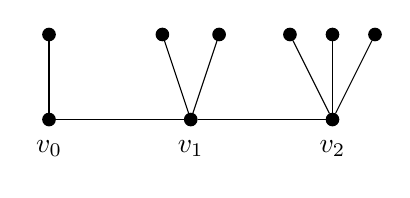
\begin{tikzpicture}[every node/.style={circle,draw,inner sep=1.6pt,fill=black},
                    scale=0.9]
   \node[label=below:{$v_0$}] (v0) at (0,0) {};
   \node[label=below:{$v_1$}] (v1) at (2,0) {};
   \node[label=below:{$v_2$}] (v2) at (4,0) {};
   \node (a)  at (0,1.2) {};
   \node (b1) at (1.6,1.2) {};
   \node (b2) at (2.4,1.2) {};
   \node (c1) at (3.4,1.2) {};
   \node (c2) at (4.0,1.2) {};
   \node (c3) at (4.6,1.2) {};
   \draw (v0) -- (v1) -- (v2);
   \draw (v0) -- (a);
   \draw (v1) -- (b1); \draw (v1) -- (b2);
   \draw (v2) -- (c1); \draw (v2) -- (c2); \draw (v2) -- (c3);
\end{tikzpicture}
\end{center}

Rather than compute the full chromatic symmetric function (which has
$2^8 = 256$ edge subsets to enumerate), we extract precisely the
coefficients required by the proof of Theorem~\ref{thm:cat}.

\paragraph{Computing $\lambda = \type(L)$.}
The set $L$ of leaf edges has cardinality $f_0+f_1+f_2 = 6$.  Removing
all spine edges from $T$ and keeping only $L$ leaves three components,
of orders $f_0+1=2,\,f_1+1=3,\,f_2+1=4$.  Hence
\[
   \lambda \;=\; (4,3,2),
   \qquad c_{\lambda}(T) = (-1)^{9-3} = +1.
\]
We verify that $\lambda$ is the unique singleton-free partition of $9$
of length $3$ with non-zero coefficient.  The other singleton-free
partitions of $9$ of length $3$ are $(5,2,2)$ and $(3,3,3)$.  By
Step~1 of the proof, every $A$ with singleton-free type contains $L$
(forcing the components to be unions of the three blocks
$\{v_0,\text{leaf}\}$, $\{v_1,\text{leaves}\}$, $\{v_2,\text{leaves}\}$
of orders $2,3,4$).  No subset of these blocks can be merged to produce
component sizes $\{5,2,2\}$ or $\{3,3,3\}$, so $c_{(5,2,2)} = c_{(3,3,3)}
= 0$.

\paragraph{Computing the $\mu_i$.}
The two spine edges are $e_1 = v_0v_1$ and $e_2 = v_1v_2$.
\begin{itemize}[leftmargin=*]
\item $L\cup\{e_1\}$ merges the components of orders $2$ and $3$,
      yielding $\mu_1 = (5,4)$.
\item $L\cup\{e_2\}$ merges the components of orders $3$ and $4$,
      yielding $\mu_2 = (7,2)$.
\end{itemize}
Both are singleton-free partitions of length $2$, and indeed
$\mu_1\neq\mu_2$.  Each contributes $(-1)^{9-2} = -1$ to its
coefficient, and (as in Step~1) no other edge subset gives a
singleton-free partition of length $2$, so
$c_{(5,4)}(T) = c_{(7,2)}(T) = -1$.

\paragraph{Reconstruction of $T$ from $\X_T$.}
Suppose we are handed only the data $\X_T$.  We extract:
\begin{enumerate}[label=(\arabic*)]
   \item By Proposition~\ref{prop:invariants}(i)--(iii), $n=9$,
         $|E(T)|=8$, and the graph has one connected component.  Hence
         it is connected with $n-1$ edges, so it is a tree on $9$
         vertices.  By Proposition~\ref{prop:invariants}(v) and Corollary~5
         of~\cite{MMW}, $\delta_1(T)=6$ leaves and the diameter is~$4$,
         from which one may verify (using
         Proposition~10 of~\cite{MMW}) that $T$ is a caterpillar.
   \item The maximum length of a singleton-free partition with
         $c_\lambda(T)\neq 0$ is $s+1 = 3$, so the spine has $3$ vertices.
   \item The unique such partition is $\lambda = (4,3,2)$, so the
         multiset of leaf numbers is $\{4-1, 3-1, 2-1\} = \{3,2,1\}$.
   \item The singleton-free partitions of $9$ of length $2$ with
         $c_\lambda(T)\neq 0$ are $(5,4)$ and $(7,2)$, so
         $\{\mu_1,\mu_2\} = \{(5,4),(7,2)\}$.
   \item Comparing $\mu_1=(5,4)$ to $\lambda=(4,3,2)$, the multiset of
         parts of $\lambda$ absent from $\mu_1$ is $\{3,2\}$.  Hence the
         endpoints of one spine edge have leaf numbers $\{3-1,2-1\}
         = \{2,1\}$.
   \item Comparing $\mu_2=(7,2)$ to $\lambda=(4,3,2)$, the missing
         parts are $\{4,3\}$, so the endpoints of the other spine edge
         have leaf numbers $\{3,2\}$.
   \item The auxiliary graph $H$ has vertex set $\{1,2,3\}$ and edges
         $\{1,2\}$ and $\{2,3\}$, which is the path $1$--$2$--$3$.
         Reading off the path gives the leaf-number sequence
         $(1,2,3)$, up to reversal.
\end{enumerate}
This recovers $T$ up to isomorphism, as predicted by
Theorem~\ref{thm:cat}.

\section{A conjecture and partial progress}\label{sec:conjecture}

The source paper proves reconstructibility for several special families of
caterpillars, including the distinct positive leaf number case treated in
Theorem~\ref{thm:cat}.  Later work proves stronger caterpillar results:
proper caterpillars are distinguished by their chromatic symmetric functions
\cite{AlistePrietoZamora}, and Loebl and Sereni prove Stanley's
isomorphism conjecture for caterpillars more generally~\cite{LoeblSereni}.
Thus the broad statement ``every caterpillar is determined by $\X_T$'' is
best regarded here as historical motivation rather than as an open conjecture.

The proof of Theorem~\ref{thm:cat}, however, suggests a sharper question
about how much of $\X_T$ is actually needed.  Let the \emph{singleton-free
coefficient data} of a tree $T$ mean the set of coefficients
$c_\lambda(T)$ for partitions $\lambda$ with no part equal to $1$.

\begin{conjecture}[Singleton-free caterpillar reconstruction]\label{conj:cat}
Let $T$ be a caterpillar whose leaf numbers $f_0,\ldots,f_s$ are all
positive.  Then the singleton-free coefficient data of $\X_T$ determines
the linear order of the multiset $\{f_0,\ldots,f_s\}$ along the spine, up
to reversal.  Equivalently, this data determines $T$ up to isomorphism
among positive caterpillars.
\end{conjecture}

\paragraph{Evidence for Conjecture~\ref{conj:cat}.}
\begin{enumerate}
\item Theorem~\ref{thm:cat} proves the conjecture when the leaf numbers
      are pairwise distinct.  In that case, the length $s+1$ singleton-free
      partition $\lambda=\type(L)$ recovers the vertex set of leaf
      numbers, and the length $s$ singleton-free partitions
      $\mu_i=\type(L\cup\{e_i\})$ recover the edge set of the path of
      leaf numbers.
\item Remark~\ref{rem:relax} gives additional positive cases when equal
      leaf numbers occur in contiguous blocks.
\item The accompanying SageMath code performs a brute-force search over
      positive caterpillars up to $12$ vertices and finds no collision in
      the singleton-free coefficient data among non-isomorphic examples.
\item The known reconstructibility of caterpillars from the full chromatic
      symmetric function~\cite{AlistePrietoZamora,LoeblSereni} supports
      the idea that the essential information may already be concentrated
      in the singleton-free part of the power-sum expansion.
\end{enumerate}

\paragraph{A partial result.}
The following proposition proves the first stage of the conjecture: the
singleton-free coefficient data determines the multiset of leaf numbers,
even if it does not yet determine their order.

\begin{proposition}\label{prop:partial}
Let $T$ be a caterpillar with spine $v_0,\ldots,v_s$ and leaf numbers
$f_0,\ldots,f_s$, and assume every $f_i\geq 1$.  Then the multiset
$\{f_0,f_1,\ldots,f_s\}$ is determined by the singleton-free coefficient
data of $\X_T$.
\end{proposition}

\begin{proof}
Let $L$ be the set of leaf edges of $T$.  As in Step~1 of the proof of
Theorem~\ref{thm:cat}, an edge set $A\subseteq E(T)$ has singleton-free
type if and only if $L\subseteq A$.  Therefore the maximum possible length
of a singleton-free type is achieved when $A=L$ and is equal to $s+1$.
Moreover, $A=L$ is the unique edge set giving singleton-free type of this
maximum length.

Thus the singleton-free coefficient data identifies the unique
singleton-free partition $\lambda$ of maximum length with nonzero
coefficient.  This partition is
\[
   \lambda=\type(L)=(f_0+1,f_1+1,\ldots,f_s+1)
\]
as a multiset of parts.  Subtracting $1$ from each part of $\lambda$
recovers the multiset $\{f_0,\ldots,f_s\}$.
\end{proof}

Proposition~\ref{prop:partial} reduces
Conjecture~\ref{conj:cat} to the problem of recovering the linear order,
up to reversal, of a known multiset of positive leaf numbers along the
spine.  The proof of Theorem~\ref{thm:cat} solves this when the leaf
numbers are distinct by using the partitions $\mu_i$.  When repeated leaf
numbers occur, several edge sets may share the same type, so one has to
control multiplicities in the coefficients $c_\mu(T)$.  This is the main
obstruction to extending the same elementary proof to all positive
caterpillars.

\section{Computational aspects}\label{sec:code}

A natural complement to the proof and examples above is a computational
verification of Theorem~\ref{thm:cat} and an exploration of
Conjecture~\ref{conj:cat}.  The accompanying SageMath file
\texttt{csf\_trees.sage} implements the following:
\begin{itemize}[leftmargin=*]
\item a routine that computes the power-sum coefficient dictionary
      $\{\lambda \mapsto c_\lambda(T)\}$ by enumerating all edge subsets
      $A\subseteq E(T)$ and applying Stanley's expansion;
\item routines that compute the connector polynomial $\K_T(x,y)$ and the
      subtree polynomial $\St_T(q,r)$ directly from the tree;
\item a verification routine for the formulas of Theorem~1 of
      Martin--Morin--Wagner, comparing the directly computed connector
      and subtree polynomials with the values obtained from the
      coefficients $c_\lambda(T)$;
\item a reconstruction routine for positive caterpillars with distinct
      leaf numbers, following the four-step proof of
      Theorem~\ref{thm:cat};
\item a brute-force search over positive caterpillars up to $12$ vertices
      that compares singleton-free coefficient data and reports whether
      any non-isomorphic examples collide.
\end{itemize}
The code takes SageMath graph objects as input.  Its output consists of
coefficient dictionaries, polynomial dictionaries, reconstructed leaf
number sequences, and collision reports.  The README supplied with the
code explains how to run the script and includes sample output for the
examples discussed in this report.

\begin{thebibliography}{99}

\bibitem{Bollobas} B.~Bollob\'as,
  \emph{Modern Graph Theory},
  Graduate Texts in Mathematics 184, Springer-Verlag, New York, 1998.

\bibitem{EisenstatGordon} D.~Eisenstat and G.~Gordon,
  \emph{Non-isomorphic caterpillars with identical subtree data},
  Discrete Math. \textbf{306} (2006), 827--830.

\bibitem{Fougere} J.~Fougere,
  \emph{On symmetric chromatic polynomials of trees},
  undergraduate thesis, Dartmouth College, 2003.

\bibitem{GordonMcDonnell} G.~Gordon and E.~McDonnell,
  \emph{Trees with the same degree sequence and path number},
  Discrete Math. \textbf{147} (1995), 297--300.

\bibitem{HeilJi} S.~Heil and C.~Ji,
  \emph{On an algorithm for comparing the chromatic symmetric functions of trees},
  Australas. J. Combin. \textbf{75} (2019), 210--222.

\bibitem{AlistePrietoZamora} J.~Aliste-Prieto and J.~Zamora,
  \emph{Proper caterpillars are distinguished by their chromatic symmetric function},
  Discrete Math. \textbf{315--316} (2014), 158--164.

\bibitem{LoeblSereni} M.~Loebl and J.-S.~Sereni,
  \emph{Isomorphism of weighted trees and Stanley's isomorphism conjecture for caterpillars},
  Ann. Inst. Henri Poincar\'e D \textbf{6} (2019), 357--384.

\bibitem{Macdonald} I.~G.~Macdonald,
  \emph{Symmetric Functions and Hall Polynomials}, 2nd ed.,
  Oxford University Press, New York, 1995.

\bibitem{MMW} J.~L.~Martin, M.~Morin, and J.~D.~Wagner,
  \emph{On distinguishing trees by their chromatic symmetric functions},
  J. Combin. Theory Ser. A \textbf{115} (2008), 237--253.

\bibitem{Morin} M.~Morin,
  \emph{Caterpillars, Ribbons, and the Chromatic Symmetric Function},
  M.S. thesis, University of British Columbia, 2005.

\bibitem{Stanley} R.~P.~Stanley,
  \emph{A symmetric function generalization of the chromatic polynomial
  of a graph},
  Adv. Math. \textbf{111} (1995), 166--194.

\bibitem{StanleyEC2} R.~P.~Stanley,
  \emph{Enumerative Combinatorics, Vol.~2},
  Cambridge University Press, Cambridge, 1999.

\bibitem{Tan} L.-Y. Tan,
  \emph{Computational verification that the chromatic symmetric
  function determines up to isomorphism trees of order at most~$23$},
  available at \url{http://www.cs.wustl.edu/~lt1/csf.html}, retrieved
  2007.

\end{thebibliography}

\end{document}
